\documentclass[a4paper,12pt]{article}
%%%%%%%%%%%%%%%%%%%%%%%%%%%%%%%%%%%%%%%%%%%%%%%%%%%%%%%%%%%%%%%%%%%%%%%%%%%%%%%%%%%%%%%%%%%%%%%%%%%%%%%%%%%%%%%%%%%%%%%%%%%%%%%%%%%%%%%%%%%%%%%%%%%%%%%%%%%%%%%%%%%%%%%%%%%%%%%%%%%%%%%%%%%%%%%%%%%%%%%%%%%%%%%%%%%%%%%%%%%%%%%%%%%%%%%%%%%%%%%%%%%%%%%%%%%%
\usepackage{eurosym}
\usepackage{vmargin}
\usepackage{amsmath}
\usepackage{graphics}
\usepackage{framed}
\usepackage{epsfig}
\usepackage{subfigure}
\usepackage{fancyhdr}

\setcounter{MaxMatrixCols}{10}
%TCIDATA{OutputFilter=LATEX.DLL}
%TCIDATA{Version=5.00.0.2570}
%TCIDATA{<META NAME="SaveForMode"CONTENT="1">}
%TCIDATA{LastRevised=Wednesday, February 23, 201113:24:34}
%TCIDATA{<META NAME="GraphicsSave" CONTENT="32">}
%TCIDATA{Language=American English}

\pagestyle{fancy}
\setmarginsrb{20mm}{0mm}{20mm}{25mm}{12mm}{11mm}{0mm}{11mm}
\lhead{MA4505} \rhead{Kevin O'Brien} \chead{Midterm
Assessment Paper 1 } %\input{tcilatex}

\begin{document}
\begin{center}
	
\includegraphics[scale=0.60]{images/shieldtransparent2}
\end{center}

\begin{center}
	\vspace{1cm}
	\large \bf {FACULTY OF SCIENCE AND ENGINEERING} \\[0.5cm]
	\normalsize DEPARTMENT OF MATHEMATICS AND STATISTICS \\[1.25cm]
	\large \bf {MID-TERM ASSESSMENT EXAMINATION 1} \\[1.0cm]
\end{center}

\begin{tabular}{ll}
%	MODULE CODE: MA4505 & SEMESTER: Autumn 2015\\[1cm]
	MODULE TITLE: Applied Statistic for Administration  & DURATION OF EXAM: 45 minutes \\[1cm]
	LECTURER: Mr. Kevin O'Brien & GRADING SCHEME: 15 marks \\
%	& \phantom{GRADING SCHEME:} \footnotesize {15\% of total module marks} \\[0.2cm]
%	\\[1cm]
\end{tabular}
\bigskip
\begin{center}
	{\bf INSTRUCTIONS TO CANDIDATES}
\end{center}

\begin{itemize} 
	\item This exam will start at 12:05, and will last 45 minutes.
	
	\item Each question will be worth either 1 or 2 Marks. There are 15 Marks worth of questions.
	\item All questions must be attempted (LENS students please see below)
	
	\item Write all of your answers in the exam script. Write the script number on any other documents you submit.
	
	\item It is your responsibility to return the script to collection box. An audit of scripts will take place immediately after the exam. If your script is account for in that audit,  you are deemed to be absent, and will receive no marks.
	
	\item \textbf{IMPORTANT for LENS Student:}
	Specifically approved LENS students have to answer any selection of questions that have an aggregate mark of 12 Marks.  
	\begin{itemize}
		\item They may skip any three of the 1-Mark Questions
		\item OR - They may skip a 1-Mark Question and a 2-Mark Question
		\item The mark will be rescaled by 125 \%.
		\item They are advised to skip questions that are indicated by an asterisk symbol (``$\ast$"), but it is not compulsory that they do so.
	\end{itemize}
	
	
\end{itemize}
\newpage
\section*{Attempt ALL questions}


Explain why an adjusted R2 value is often preferred to R2
when comparing
models. 

%- http://www.hkss.org.hk/images/exam/papers/Past/2009/2009_GD_M4_HKSS.pdf



%=============================================================%
Usual assumptions are that the residual (error) terms should be independent,
identically distributed, have zero mean and constant variance, and, if the usual
inferences and tests are to be made, be Normally distributed. 


%-------------------------------------------------------------%
\newpage
%\subsubsection*{Regression ANOVA}
\subsubsection*{Question 3 Part B (6 Marks)}
Suppose we have a regression model, described by the following equation
\[ \hat{y} = 28.81 + 6.45x_1 + 7.82 x_2\]
We are given the following pieces of information.
\begin{itemize}
	\item The standard deviation of the response variance $y$ is 10 units.
	\item There are 53 observations.
	\item The \textit{Coefficient of Determination} (also known as the \textit{Multiple R-Squared}) is 0.75.
\end{itemize}
Complete the \textit{Analysis of Variance} Table for a linear regression model.
The required values are indicated by question marks.

\begin{center}
	\begin{tabular}{|c|c|c|c|c|c|} \hline
		\phantom{makespace}	& DF & 	Sum Sq &	Mean Sq &	F value &   	Pr($>$F)    \\ \hline
		Regression &  \phantom{make}?\phantom{make} &	? &	? &	 ? &	$< 2.2e^{-16}$ \\ \hline
		Error  & ? &	? &  	?   &            &       \\ \hline
		Total  & ?  &	? &  \phantom{makespace}	  &   \phantom{makespace}         &    \phantom{makespace}    \\ \hline
	\end{tabular} 
\end{center}
	\subsection*{Question 1 Inference Procedures}
	
	%	\begin{framed}
	%		What is going here?
	%		\begin{itemize}
	%			\item Using the Murdoch Barnes Table for Normal Distribution Problems
	%			\item Testing that Data is normally distributed (may appear elsewhere)
	%			\item Transformation of Data (Tukey's Ladder)
	%			\item Outliers and Boxplots (Grubbs Test, Dixon Q-test)
	%			\item Non-Parametric Procedures (e.g. Wilcoxon test, Kolmogorov Smirnov Test)
	%		\end{itemize}
	%	\end{framed}
	%\newpage
	%\subsubsection*{Question 1 Part A (4 Marks)}
	%%\subsubsection*{Part A Theory for Inference Procedures (4 Marks)}
	%Answer the four short questions. Each correct answer will be awarded 1 mark.
	%\begin{itemize}
	%	\item[(i.)] What is a $p-$value?
	%	\item[(ii.)] Briefly describe how $p-$value is used in hypothesis testing.
	%	\item[(iii.)] What is meant by a Type I error?
	%	\item[(iv.)] What is meant by a Type II error?
	%\end{itemize}
	\subsubsection*{Question 1 Part A (5 Marks)}
	Numeric Transformations, such as logarithmic transformation, are often used in statistical analysis as an approach for dealing with non-normal data.
	\begin{itemize}
		\item[(i)] (1 Marks) Discuss the importance of numeric transformations, such as logarithmic transformation, in Statistics.
		\item[(ii)] Describe the process of transformations
		\item[(i.)] (1 Mark) Describe the purpose of Tukey's Ladder (referencing direction and relative strength).
		\item[(ii.)] (2 Marks) Give two examples of a transformation for various types of skewed data (i.e. an example for both types of skewness).
		\item[(iii.)] (1 Mark) Discuss the limitations of numeric transformations.
	\end{itemize}
	

\bigskip

\subsubsection*{Part C - Robust Regression (7 Marks)}

% \subsection*{Q9.Robust Regression}
%Write a brief explanation of how robust regression differs from linear models computed using the \emph{Ordinary Least Squares method}, making reference to one particular weighting method only. Provide a description on how this weighting method works.


In certain circumstances, Robust Regression may be used in preference to Ordinary Least Squares Regression. Answer the following questions relating to Robust Regression. 

\begin{itemize}
	\item[(i.)] (1 Mark) Describe what these circumstances might be.
	\item[(ii.)] (1 Mark) State one difference between OLS and Robust regression techniques, in terms of computing regression equations.
	\item[(iii.)] (2 Marks) Explain the process of Huber Weighting for Residuals, stating the algorithm used to compute weightings.
	\item[(iv.)] (3 Marks) Suppose that Huber Weighting, with a tuning constanct of $k=13.45$, was applied to the observations 
	tabulated below. What would be the outcome of the procedure for each case. 
\end{itemize}
\begin{center}
	\begin{tabular}{|c|c|}
		\hline
		Observation & Residual \\ 
		$i$  & $e_i$ \\ \hline
		11 & -9.07 \\ \hline 
		14 & 14.54 \\ \hline
		18 & 22.91 \\ \hline
	\end{tabular} 
\end{center}	
	\subsubsection*{Question 1 Part B (5 Marks)}
	
	The typing speeds for one group of 12 Engineering students were recorded both at the beginning of year 1 of their studies. The results (in words per minute) are given below:
	
	\begin{center}
		\begin{tabular}{|c|c|c|c|c|c|}
			\hline
			% Subject& A& B& C& D& E &F &G &H \\ \hline
			149  & 146 & 112 & 142 & 168& 153\\ \hline
			137 & 161 & 156& 165&  170&  159
			\\ \hline
		\end{tabular}
	\end{center}
	Use the Dixon Q-test to determine if the lowest value (118) is an outlier. You may assume a significance level of 5\%.
	\begin{itemize}
		\item[(i.)](1 Mark)	State the Null and Alternative Hypothesis for this test.
		\item[(ii.)](2 Marks) Compute the test statistic
		\item[(iii.)](1 Mark) State the appropriate critical value.
		\item[(iv.)](1 Mark) What is your conclusion to this procedure.
	\end{itemize}
	\newpage
	\subsubsection*{Question 1 Part C (5 Marks)}
	
	%\subsubsection*{Part A : Outliers}
	\begin{itemize}
		\item[(i.)] (3 Marks) Provide a brief description for three tests from the family of Grubb's  Outliers Tests. Include in your description a statement of the null and alternative hypothesis for each test
		\item[(ii.)] (2 Marks) Describe any required assumptions for tests, and the limitations of these tests.
	\end{itemize}
	
	
	
	% Review of Univariate Normal Distribution
	% Test for Univariate normality
	% - Graphical Procedures
	% - Formal Tests
	% (Later Multivariate Normality)
	% Boxplots, Outliers and Transformations
	%
	% (Hint: there are no outliers in these data sets)
	
	\bigskip
	%--------------------------------------------------------------------------------------- %
	\subsubsection*{Question 1 Part D (10 Marks)}
	% Normal %6 MARKS
	Assume that the diameter of a critical component is normally distributed with a mean of 250mm and a standard deviation of 15mm. You are required  to estimate the approximate probability of the following measurements occurring on an individual component.
	\begin{itemize}
		\item[(i.)](3 Mark) Greater than 245mm.
		\item[(ii.)](3 Marks) Less than 265mm.
		\item [(iii.)](4 Marks) Between 245mm and 265mm.
	\end{itemize}
	\bigskip
	\noindent Use the normal tables to determine the probabilities for the above exercises. You are required to show all of your workings.
	
	
	%====================================================================== %
	\newpage
\subsection*{Question 4. Linear Models (25 Marks)}
\subsubsection*{Question 4 Part A (12 Marks)}
The mercury level of several tests of sea-water from costal areas was determined by atomic-absorption spectrometry. The results obtained are as follows

%\begin{figure}[h!]
%	\centering
%	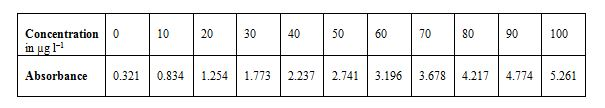
\includegraphics[width=1.1\linewidth]{image/regressionData}
%\end{figure}

The analysis of the relationship between concentration and absorbance is obtained in R and presented below. 
\begin{framed}
	\begin{verbatim}
	x<-seq(0,100,by=10)
	y<- c(0.321, 0.834, 1.254, 1.773, 2.237, 2.741, 3.196, 3.678, 
	4.217, 4.774, 5.261)
	model<- lm(y~x)
	summary(model)
	
	Call:
	lm(formula = y ~ x)
	
	Coefficients:
	Estimate Std. Error t value Pr(>|t|)    
	(Intercept) 0.2933636  0.0234754   12.50 5.45e-07 
	x           0.0491982  0.0003968  123.98 7.34e-16 
	---
	
	Residual standard error: 0.04162 on 9 degrees of freedom
	Multiple R-squared: 0.9994,     Adjusted R-squared: 0.9993 
	F-statistic: 1.537e+04 on 1 and 9 DF,  p-value: 7.337e-16 
	
	confint(model)
	2.5 %     97.5 %
	(Intercept) 0.24025851 0.34646876
	x           0.04830054 0.05009582
	
	\end{verbatim}
\end{framed}
\newpage
\begin{itemize}
	\item[(i)] (2 marks)
	Determine and interpret the slope and the intercept of the regression line.
	\item[(ii)]  (2 marks) State the 95\% confidence interval for the slope and the intercept coefficients. Interpret this intervals with respect to any relevant hypothesis tests
	\item[(iii)] (2 marks) Explain in which way is the prediction intervals different from the confidence intervals for fitted values in linear regression?
	\item[(iv)] (2 Marks) The following piece of \texttt{R} code gives us a statistical metric. What is this metric? What is it used for? How should it be interpreted.
	
\end{itemize}
\begin{framed}
	\begin{verbatim}
	> AIC(model)
	[1] -34.93389	
	\end{verbatim}
\end{framed}

%=====================================================

%Write a short note to compare and contrast the multiple R squared and asjusted R squared.
%%% - Overfitting

%====================================================================== %
\newpage

\subsubsection*{Question 4 Part B (12 Marks)}

%\subsubsection*{Model Selection}
Given the AIC for each candidate model, use \textbf{\textit{Backward Selection}} to determine the optimal model for predicting values of $y$ with predictor variables
$x_1$, $x_2$,$x_3$ and $x_4$.

Suppose we have 5 predictor variables.
Use \textbf{Forward Selection} and \textbf{Backward Selection} to choose the optimal set of predictor variables, based on the AIC measure.

{
	\large
	\begin{center}
		\begin{tabular}{||c|c||c|c||}
			\hline
			Variables & AIC & Variables & AIC \\ \hline \hline
			$\emptyset$	&	200	&	x1, x2, x3	&	74	\\ \hline
			\phantom{makemakespace}
			&	\phantom{makespace}
			&	x1, x2, x4	&	75	\\ \hline
			x1	&	150	&	x1, x2, x5	&	79	\\ \hline
			x2	&	145	&	x1, x3, x4	&	72	\\ \hline
			x3	&	135	&	x1, x3, x5	&	85	\\ \hline
			x4	&	136	&	x1, x4, x5	&	95	\\ \hline
			x5	&	139	&	x2, x3, x4	&	83	\\ \hline
			&		&	x2, x3, x5	&	82	\\ \hline
			x1, x2	&	97	&	x2, x4, x5	&	78	\\ \hline
			x1, x3	&	81	&	x3, x4, x5	&	85	\\ \hline
			x1, x4	&	94	&	\phantom{makemakespace}
			&	\phantom{makespace}
			\\ \hline
			x1, x5	&	88	&	x1, x2, x3, x4	&	93	\\ \hline
			x2, x3	&	87	&	x1, x2, x3, x5	&	120	\\ \hline
			x2, x4	&	108	&	x1, x2, x4, x5	&	104	\\ \hline
			x2, x5	&	87	&	x1, x3, x4, x5	&	101	\\ \hline
			x3, x4	&	105	&	x2, x3, x4, x5	&	89	\\ \hline
			x3, x5	&	82	&		&		\\ \hline
			x4, x5	&	86	&	x1, x2, x3, x4, x5	&	100	\\ \hline
		\end{tabular} 
	\end{center}
}
%================================================= %
\newpage
%\subsubsection*{Regression ANOVA}
\subsubsection*{Question 3 Part B (6 Marks)}
Suppose we have a regression model, described by the following equation
\[ \hat{y} = 28.81 + 6.45x_1 + 7.82 x_2\]
We are given the following pieces of information.
\begin{itemize}
	\item The standard deviation of the response variance $y$ is 10 units.
	\item There are 53 observations.
	\item The \textit{Coefficient of Determination} (also known as the \textit{Multiple R-Squared}) is 0.75.
\end{itemize}
Complete the \textit{Analysis of Variance} Table for a linear regression model.
The required values are indicated by question marks.

\begin{center}
	\begin{tabular}{|c|c|c|c|c|c|} \hline
		\phantom{makespace}	& DF & 	Sum Sq &	Mean Sq &	F value &   	Pr($>$F)    \\ \hline
		Regression &  \phantom{make}?\phantom{make} &	? &	? &	 ? &	$< 2.2e^{-16}$ \\ \hline
		Error  & ? &	? &  	?   &            &       \\ \hline
		Total  & ?  &	? &  \phantom{makespace}	  &   \phantom{makespace}         &    \phantom{makespace}    \\ \hline
	\end{tabular} 
\end{center}


\newpage
%======================================================


\section*{Polynomial Regression}
\begin{itemize}
	\item Polynomial regression models are useful in situations where the analyst knows that \textit{\textbf{curvilinear effects}} are present in the response variable.
	\item Polynomial models are also useful as approximating functions to unknown and possible very complex nonlinear relationship.
\end{itemize}


In the context of Statistical Modelling, what is means the ``Law of Parsimony".

What is the Akaike information criterion? How would you use it in statical modelling? How does it differ from other metrics such as the 
coefficient of determination. How would you interpret an AIC value.

compare and contrast forward selection and backward selection as variable selection procedures.

In the context of Statistical Modelling,What is meant by Stepwise regression?

Explain why an adjusted R2 value is often preferred to R2
when comparing
models. 

%- http://www.hkss.org.hk/images/exam/papers/Past/2009/2009_GD_M4_HKSS.pdf



%=============================================================%
Usual assumptions are that the residual (error) terms should be independent,
identically distributed, have zero mean and constant variance, and, if the usual
inferences and tests are to be made, be Normally distributed. 


%-------------------------------------------------------------%
\newpage



\subsection*{Q2. Testing Normality (3 Marks)} %4 Marks
A graphical procedure was carried out to assess whether or not this assumption of normality is valid for data set \texttt{Y}. Consider the Q-Q plot in the figure below.

\begin{center}
	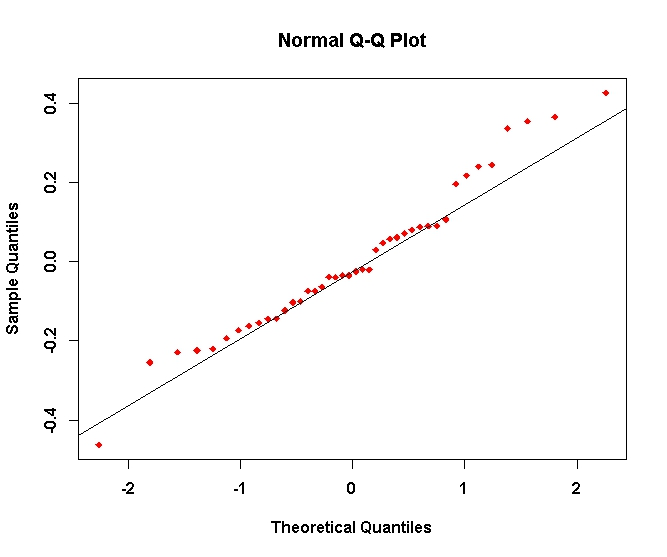
\includegraphics[scale=0.45]{images/ExamQ5qqplot}
\end{center}

\begin{itemize}
	\item[i.] (1 Mark) Provide a brief description on how to interpret this plot.
	\item[ii.] (1 Mark) What is your conclusion for this procedure? Justify your answer.
\end{itemize}

\subsection*{Q3. Testing Normality (4 Marks)} %4 Marks
Consider the following inference procedure performed on data set $X$.
\begin{center}
	\begin{verbatim}
	> shapiro.test(X)
	
	Shapiro-Wilk normality test
	
	data:  X
	W = 0.8914, p-value = 0.07047
	
	\end{verbatim}
\end{center}


\begin{itemize}
	\item[i.] (1 Mark) Describe what is the purpose of this procedure.
	\item[ii.] (1 Mark) What is the null and alternative hypothesis?
	\item[iii.] (1 Mark) Write the conclusion that follows from it.
	\item[iv.] (1 Mark) Tests for Normality are known to be susceptible to low power. Discuss what is meant by this.
\end{itemize}


\subsection*{Q4. Dixon Q Test For Outliers (4 Marks)}

The typing speeds for one group of 12 Engineering students were recorded both at the beginning of year 1 of their studies. The results (in words per minute) are given below:

\begin{center}
	\begin{tabular}{|c|c|c|c|c|c|c|}
		\hline
		% Subject& A& B& C& D& E &F &G &H \\ \hline
		121 & 146 & 150 &149 &142 &170& 153\\ \hline
		137 & 161 & 156& 165& 137& 178& 159
		\\ \hline
	\end{tabular}
\end{center}
Use the Dixon Q-test to determine if the lowest value (121) is an outlier. You may assume a significance level of 5\%.
%Calculate a 95\% confidence interval for the difference between the mean number of marks obtained by males and females in the population of school leavers as a whole.
%(7 marks)

\begin{itemize}
	\item[i.] (1 Mark) Formally state the null hypothesis and the alternative hypothesis.
	\item[ii.] (1 Mark) Compute the Test Statistic.
	\item[iii.] (2 Mark) By comparing the Test Statistic to the appropriate Critical Value, state your conclusion for this test.
\end{itemize}


\bigskip
\subsection*{Q1. Dixon Q Test For Outliers (4 Marks)}

The typing speeds for one group of 12 Engineering students were recorded both at the beginning of year 1 of their studies. The results (in words per minute) are given below:

\begin{center}
	\begin{tabular}{|c|c|c|c|c|c|}
		\hline
		% Subject& A& B& C& D& E &F &G &H \\ \hline
		118 & 146 & 149 & 142 & 170& 153\\ \hline
		137 & 161 & 156& 165&  178& 159
		\\ \hline
	\end{tabular}
\end{center}
Use the Dixon Q-test to determine if the lowest value (118) is an outlier. You may assume a significance level of 5\%.
\begin{itemize}
	\item[i.](1 Mark)	State the Null and Alternative Hypothesis for this test.
	\item[ii.](1 Marks) Compute the test statistic
	\item[iii.](1 Mark) State the appropriate critical value.
	\item[iv.](1 Mark) What is your conclusion to this procedure
\end{itemize}

%Calculate a 95\% confidence interval for the difference between the mean number of marks obtained by males and females in the population of school leavers as a whole.
%(7 marks)

\newpage
%\newpage


\section*{Formulae and Tables}
\subsection*{Critical Values for Dixon Q Test}
{
	\Large
	\begin{center}
		\begin{tabular}{|c|c|c|c|}
			\hline  N  & $\alpha=0.10$  & $\alpha=0.05$  & $\alpha=0.01$  \\ \hline
			3  & 0.941 & 0.970 & 0.994 \\ \hline
			4  & 0.765 & 0.829 & 0.926 \\ \hline
			5  & 0.642 & 0.710  & 0.821 \\ \hline
			6  & 0.560 & 0.625 & 0.740 \\ \hline
			7  & 0.507 & 0.568 & 0.680  \\ \hline
			8  & 0.468 & 0.526 & 0.634 \\ \hline
			9  & 0.437 & 0.493 & 0.598 \\ \hline
			10 & 0.412 & 0.466 & 0.568 \\ \hline
			11 & 0.392 & 0.444 & 0.542 \\ \hline
			12 & 0.376 & 0.426 & 0.522 \\ \hline
			13 & 0.361 & 0.410 & 0.503 \\ \hline
			14 & 0.349 & 0.396 & 0.488 \\ \hline
			15 & 0.338 & 0.384 & 0.475 \\ \hline
			16 & 0.329 & 0.374 & 0.463 \\ \hline
		\end{tabular} 
	\end{center}
}
\newpage
\subsection*{Critical Values for Chi Square Test}
{



\end{document}
\subsection*{Confidence Intervals}
{\bf One sample}
\begin{eqnarray*} S.E.(\bar{X})&=&\frac{\sigma}{\sqrt{n}}.\\\\
S.E.(\hat{P})&=&\sqrt{\frac{\hat{p}\times(100-\hat{p})}{n}}.\\
\end{eqnarray*}
{\bf Two samples}
\begin{eqnarray*}
S.E.(\bar{X}_1-\bar{X}_2)&=&\sqrt{\frac{\sigma^2_1}{n_1}+\frac{\sigma_2^2}{n_2}}.\\\\
S.E.(\hat{P_1}-\hat{P_2})&=&\sqrt{\frac{\hat{p}_1\times(100-\hat{p}_1)}{n_1}+\frac{\hat{p}_2\times(100-\hat{p}_2)}{n_2}}.\\\\
\end{eqnarray*}
\subsection*{Hypothesis tests}
{\bf One sample}
\begin{eqnarray*}
S.E.(\bar{X})&=&\frac{\sigma}{\sqrt{n}}.\\\\
S.E.(\pi)&=&\sqrt{\frac{\pi\times(100-\pi)}{n}}
\end{eqnarray*}
{\bf Two large independent samples}
\begin{eqnarray*}
S.E.(\bar{X}_1-\bar{X}_2)&=&\sqrt{\frac{\sigma^2_1}{n_1}+\frac{\sigma_2^2}{n_2}}.\\\\
S.E.(\hat{P_1}-\hat{P_2})&=&\sqrt{\left(\bar{p}\times(100-\bar{p})\right)\left(\frac{1}{n_1}+\frac{1}{n_2}\right)}.\\
\end{eqnarray*}
{\bf Two small independent samples}
\begin{eqnarray*}
S.E.(\bar{X}_1-\bar{X}_2)&=&\sqrt{s_p^2\left(\frac{1}{n_1}+\frac{1}{n_2}\right)}.\\\\
s_p^2&=&\frac{s_1^2(n_1-1)+s_2^2(n_2-1)}{n_1+n_2-2}.\\
\end{eqnarray*}
{\bf Paired sample}
\begin{eqnarray*}
S.E.(\bar{d})&=&\frac{s_d}{\sqrt{n}}.\\\\
\end{eqnarray*}
{\bf Standard Deviation of case-wise differences (computational formula)}
\begin{eqnarray*}
s_d = \sqrt{ {\sum d_i^2 - n\bar{d}^2 \over n-1}}.\\\\
\end{eqnarray*}
\end{document}
% -- Part 3 - Confidence Interval

% 2 Marks Using previously calculated values, compute the confidence interval
